\documentclass[10pt]{beamer}

%% Chinese support
%% \usepackage[adobefonts,nocap]{ctex}

%% Fonts
\usepackage{multicol}
\usepackage{mathabx}
\usepackage[scaled]{helvet}
\usepackage{lmodern}
\usepackage{eulervm}
\usefonttheme[onlymath]{serif}
\usefonttheme{professionalfonts}
\usefonttheme{structurebold}
\usepackage{bm}
\usepackage{verbatim}

%% Color & Theme
\definecolor{SUblue}{RGB}{0,0,180}
\usecolortheme[RGB={0,0,180}]{structure}
\usetheme{Boadilla}
\setbeamertemplate{navigation symbols}{}
\setbeamertemplate{itemize items}[circle]
\setbeamertemplate{enumerate items}[circle]
\setbeamerfont{title}{size=\large}
\setbeamerfont{frametitle}{size=\large}
\setbeamerfont{framesubtitle}{size=\large,shape =$\color{violet}{\looparrowdownright}~$}
\setbeamercolor{title}{fg=white, bg= SUblue!75!green}
\setbeamercolor{framesubtitle}{fg=violet}
% \setlength{\leftmargini}{5pt}


\title[Statistical Computing]{{\textbf{Bayesian Inference with MCMC}}}

\author[Feng Li]{
\includegraphics[height=2cm]{cufelogo}\\
  \vspace{0.5cm}\textbf{Feng Li\\\texttt{feng.li@cufe.edu.cn}}}

\institute[SAM.CUFE.EDU.CN]{\footnotesize{\textbf{School of Statistics and Mathematics\\
      Central University of Finance and Economics}}}
\date{}
%%%%%%%%%%%%%%%%%%%%%%%%%%%%%%%%%%%%%%%%%%%%%%%%%%%%%%%%%%%%%%%%%%%%%%
\begin{document}

%% Title page
\begin{frame}[plain]
  \titlepage
  \tiny{Revised on \today}
\end{frame}







\section{Classical v Bayesian}
\begin{frame}{Inference}
  \begin{itemize}
  \item Let's consider a simple problem of inference.

  \item Suppose I am interested in the {\bf proportion} of students in this class who are born in Beijing.  This will be denoted as $\theta$

  \item In particular, I am interested in whether {\bf half} of the class is born in Beijing ($\theta=0.5$) or whether it is less than half ($\theta<0.5$).

  \item I am unable to ask everybody in the class if they were born in Beijing, I can only take a sample.
  \end{itemize}
\end{frame}
\begin{frame}{Classical Framework}
  \begin{itemize}
  \item In the {\bf classical framework} $\theta$ is NOT a random variable.  It is a fixed number that is unknown.

  \item Using the sample, an estimate $\hat{\theta}$ can be obtained.

  \item A 95\% confidence interval around $\hat{\theta}$ can be constructed

  \item The null hypothesis $\theta=0.5$ can be tested against the alternative $\theta< 0.5$
  \end{itemize}
\end{frame}
\begin{frame}{Intepretation in Classical Framework}
  \begin{itemize}
  \item Suppose the 95\% confidence interval is (0.3-0.45).  How is this interpreted?

  \item Correct (classical) interpretation:

    \begin{itemize}
    \item If an infinite number of samples is taken, 95\% of the confidence intervals constructed in this way will contain the true value $\theta$.
    \end{itemize}

  \item Incorrect (classical) interpretation:

    \begin{itemize}

      {
      \item {There is a 95\% probability that $\theta$ is in the interval 0.35-0.45.}
      }
      {
      \item There is a 95\% probability that $\theta$ is in the interval 0.35-0.45.
      }
    \end{itemize}

  \item Reason: $\theta$ is not a random variable.
  \end{itemize}
\end{frame}
\begin{frame}{Intepretation in Classical Framework}
  \begin{itemize}
  \item Suppose $\hat{\theta}=0.4$ and the Null is rejected at the 5\% level of significance.

  \item Correct (classical) interpretation:

    \begin{itemize}
    \item If the null were true than the probability of observing $\hat{\theta}\leq 0.4$ is less than the level of significance (5\%).  Therefore the null is rejected and we conclude  $\hat{\theta}\leq 0.5$
    \end{itemize}

  \item Incorrect (classical) interpretation:

    \begin{itemize}

      {
      \item {The probability that $\theta\leq 0.5$ is 95\%.}
      }
      {
      \item The probability that $\theta\leq 0.5$ is 95\%.
      }
    \end{itemize}

  \item Reason: $\theta$ is not a random variable.
  \end{itemize}
\end{frame}
\begin{frame}{Bayesian Framework}
  \begin{itemize}
  \item There is another way to do statistical inference known as the {\bf Bayesian Framework}.

  \item It relies on a very different understanding of probability.

  \item In the Bayesian framework probability distributions represent uncertainty about quantities that are unknown.

  \item In our example, under the Bayesian framework $\theta$ IS a random variable.
  \end{itemize}
\end{frame}
\begin{frame}{Why Bayes?}
  \begin{itemize}
  \item Let ${\bm y}=(y_1,y_2,\ldots,y_n)'$ be the data in the sample, and $\theta$ be the unknown parameter of interest.

  \item Inferences about $\theta$ are based on the distribution $p(\theta|{\bm y})$.  This can be found using Bayes' Rule

    \begin{equation}
      p(\theta|{\bm y})=\frac{p({\bm y}|\theta)p(\theta)}{p({\bm y})}
    \end{equation}

  \item Consider each term in the equation
  \end{itemize}
\end{frame}
\begin{frame}{Posterior Distribution}
  \begin{itemize}
  \item The term $p(\theta|{\bm y})$ is called the {\bf posterior distribution}.

  \item The word `posterior' comes from a Latin word meaning `after'

  \item This represents our belief about $\theta$ after seeing the data.

  \item All inference is based on this quantity.
  \end{itemize}
\end{frame}
\begin{frame}{Likelihood}
  \begin{itemize}
  \item The term $p({\bm y}|\theta)$ is called the {\bf likelihood}.

  \item This should be familiar since it is the same `likelihood' used in maximum likelihood.

  \item This represents our belief about how the data are generated for a given value of $\theta$.

  \item In the example about students born in Beijing, it will be a Bernoulli distribution.
  \end{itemize}
\end{frame}
\begin{frame}{Normalising Constant}
  \begin{itemize}
  \item The term $p({\bm y})$ can be found using the formula

    \begin{equation}
      p({\bm y})=\int_{\theta}p({\bm y},\theta)d\theta=\int_{\theta}p({\bm y}|\theta)p(\theta)d\theta
    \end{equation}

  \item However, since this term does not contain $\theta$ it forms part of the normalising constant of $p(\theta|{\bm y})$

  \item Sometimes we write Bayes Rule as:

    \begin{equation}
      p(\theta|{\bm y})\propto p({\bm y}|\theta)p(\theta)
    \end{equation}
  \end{itemize}
\end{frame}
\begin{frame}{The Prior}
  \begin{itemize}
  \item The term $p(\theta)$ is called the {\bf prior distribution}.

  \item The word `prior' comes from a Latin word meaning `before'

  \item This represents our belief about $\theta$ before seeing the data.

  \item This is the most controversial part of the Bayesian Framework
  \end{itemize}
\end{frame}
\begin{frame}{Uniform Prior}
  \begin{itemize}
  \item Suppose I know nothing about the proportion of students born in Beijing before I collect data.

  \item In this case $p(\theta)\sim U(0,1)$.

  \item Since the University is in Beijing, I could place less weight on $p(\theta)$ close to 0.

  \item Since Zhong Cai is a good university it attracts students from all of China. I could also place less weight on $p(\theta)$ close to 1.

  \item However, I will use the assumption $p(\theta)\sim U(0,1)$.
  \end{itemize}
\end{frame}
\begin{frame}{Computing the posterior}
  Let $y_i=1$ if the student is born in Beijing and $y_i=0$ otherwise:
  \begin{align}
    p(\theta|{\bm y})&\propto p({\bm y}|\theta)p(\theta)\\
                     &\prod_{i=1}^n \theta^{y_i}(1-\theta)^{(1-y_i)}\times 1\\
                     &\theta^{\sum\limits_{i=1}^ny_i}(1-\theta)^{\sum\limits_{i=1}^n(1-y_i)}\\
                     &\theta^{\sum\limits_{i=1}^ny_i}(1-\theta)^{n-\sum\limits_{i=1}^n(y_i)}
  \end{align}
  Does this look familiar?
\end{frame}
\begin{frame}{Normalizing Constant and Kernel}
  What are the
  { normalizing constant}{{\color{blue} normalizing constant}}
  and
  {kernel}{{\color{red} kernel}}
  of the Beta density?
  {
    \begin{equation}
      \mbox{Beta}(x;a,b)=\frac{\Gamma(a+b)}{(\Gamma(a)\Gamma(b))}x^{a-1}(1-x)^{b-1}
    \end{equation}
  }{
    \begin{equation}
      \mbox{Beta}(x;a,b)={\color{blue}\frac{\Gamma(a+b)}{(\Gamma(a)\Gamma(b))}}{\color{red}x^{a-1}(1-x)^{b-1}}
    \end{equation}
  }

\end{frame}

\begin{frame}{Matching}
  \begin{itemize}
  \item The kernel of the $x\sim\mbox{Beta}(a,b)$ is


    {\begin{equation}
        {\color{blue} x}^{{\color{red} a-1}}(1-{\color{blue} x})^{{\color{magenta} b-1}}
        \label{eq:betgen}
      \end{equation}}
    \begin{equation}
      x^{a-1}(1-x)^{b-1}
      \label{eq:betgen}
    \end{equation}

  \item The kernel of the posterior $p(\theta|y)$

    \begin{equation}
      {\color{blue} \theta}^{{\color{red}\sum\limits_{i=1}^ny_i}}(1-{\color{blue} \theta})^{{\color{magenta} n-\sum\limits_{i=1}^n(y_i)}}
      \label{eq:betpost}
    \end{equation}

    \begin{equation}
      \theta^{\sum\limits_{i=1}^ny_i}(1-\theta)^{n-\sum\limits_{i=1}^n(y_i)}
      \label{eq:betpost}
    \end{equation}

  \item Match $x$ in Equation~\ref{eq:betgen} with $\theta$ in Equation~\ref{eq:betpost}. What about $a$ and $b$?

  \end{itemize}
\end{frame}

\begin{frame}{Posterior}
  \begin{itemize}
  \item Match $a-1$ in Equation~\ref{eq:betgen} with $\sum\limits_{i=1}^ny_i$ in Equation~\ref{eq:betpost}

  \item Match $b-1$ in Equation~\ref{eq:betgen} with $n-\sum\limits_{i=1}^ny_i$ in Equation~\ref{eq:betpost}

  \item The posterior is
    \begin{equation}
      \theta|y\sim\mbox{Beta}\left(\sum\limits_{i=1}^ny_i+1,n-\sum\limits_{i=1}^ny_i+1\right)
    \end{equation}
  \end{itemize}
\end{frame}
\begin{frame}{Inference}
  \begin{itemize}
  \item In classical inference there is {\bf Confidence Interval}

  \item In Bayesian inference there is a similar idea called {\bf Credible Interval}

  \item Find the quantiles at 2.5\% and 97.5\% to form a 95\% credible interval

  \item You can do this in R using {\em qbeta}.

  \item How do we intepret a 95\% credible interval $(L,U)$?

  \item It is just $\mbox{Pr}\left(L\leq\theta\leq U\right)=0.95$
  \end{itemize}
\end{frame}
\begin{frame}{Point Estimates}
  \begin{itemize}
  \item Suppose we want a single estimate for $\theta$.  There
    are a few choices.

    \begin{itemize}

    \item Posterior Median $\theta^*: \int\limits_{0}^{\theta^*}p(\theta|{\bm y})d\theta=0.5$

    \item Posterior Mode: $argmax_\theta p(\theta|{\bm y})$

    \item Posterior Mean: $E_{\theta|{\bm y}}[\theta]$
    \end{itemize}

  \item For the Beta distribution, you can look these up in a textbook.

  \item Can you work out the posterior median and posterior mode using R?

  \item Can you approximate the posterior mean using R?
  \end{itemize}
\end{frame}
\begin{frame}{Testing}
  \begin{itemize}
  \item In the Classical framework there is the concept of a Hypothesis test.

  \item For example $H_0:\theta=0.5$ $H_1:\theta<0.5$

  \item In the Bayesian framework just look at posterior probabilities.

  \item For example $\mbox{Pr}(\theta<0.5)$
  \end{itemize}
\end{frame}
\begin{frame}{Classical v Bayesian}
  \begin{itemize}
  \item Many statisticians argue about whether the Classical or Bayesian framework is correct.

  \item Regardless of which one you think is correct, you should understand both.

  \item In particular you should understand how to make interpretations in both frameworks.

  \item The most important distinction is that parameters are NOT random variables in the classical framework but parameters ARE random variables in the Bayesian framework.
  \end{itemize}
\end{frame}
\section{Inference for Gaussian Data}
\begin{frame}{Gaussian Data}
  \begin{itemize}
  \item Suppose we would like to conduct Bayesian inference on the average height of adult males in a country.

  \item The observations are iid $y_i\sim N(\mu,\sigma^2)$.

  \item For now just consider inference on the average height treating the variance of height $\sigma^2$ as known.  We want $p(\mu|y,\sigma^2)$.

  \item What is a reasonable prior on $\mu$?
  \end{itemize}
\end{frame}
\begin{frame}{Prior on $\mu$}
  \begin{itemize}
  \item The prior $p(\mu)$ can also be normally distributed $\mu\sim N(\eta,\tau^2)$

  \item Different sets of values of $\eta$ and $\tau^2$ can be used.

    \begin{itemize}
    \item $p(\mu)\sim N(1.8,0.01)$
    \item $p(\mu)\sim N(1.74,0.0025)$
    \item $p(\mu)\sim N(1.78,0)$
    \item $p(\mu)\sim N(\eta,\tau^2)\quad\tau^2\rightarrow\infty$
    \end{itemize}

  \item These represent prior beliefs before we see any data.
  \item Let the the prior on $\mu$ be independent of $\sigma^2$.  We say  $\mu$ and $\sigma^2$ are  {\bf independent a priori}.
  \end{itemize}
\end{frame}
\begin{frame}{What will be the posterior?}
  \begin{itemize}
  \item The prior is $N(\eta,\tau^2)$

  \item The likelihood is $N(\mu,\sigma^2)$

  \item Maybe the posterior is also normal $N(a,b)$?

  \item What does the kernel of the normal look like?
  \end{itemize}
\end{frame}
\begin{frame}{Kernel of the Normal}
  \begin{align*}
    p(x)&=(2\pi b)^{-1/2}exp\left\{-\frac{1}{2}\left[\frac{(x-a)^2}{b}\right]\right\}\\
        &\propto exp\left\{-\frac{1}{2}\left[\frac{(x-a)^2}{b}\right]\right\}\\
        &\propto exp\left\{-\frac{1}{2}\left[\frac{(x^2-2ax+a^2}{b}\right]\right\}\\
        &\propto exp\left\{-\frac{1}{2}\left[\frac{(x^2-2ax}{b}\right]\right\}
          exp\left\{-\frac{1}{2}\left[\frac{a^2}{b}\right]\right\}\\
        &\propto exp\left\{-\frac{1}{2}\left[\frac{(x^2-2ax}{b}\right]\right\}
  \end{align*}
\end{frame}
\begin{frame}{Obtain Posterior}
  \begin{align*}
    p(\mu|{\bm y},\sigma^2) &\propto p({\bm y}|\mu,\sigma^2)p(\mu|\sigma^2)\\
                            &\propto p({\bm y}|\mu,\sigma^2)p(\mu)\\
                            &\propto \left(\prod\limits_{i=1}^nexp\left\{-\frac{1}{2}\left[\frac{\left(y_i-\mu\right)^2}{\sigma^2}\right]\right\}\right)
                              exp\left\{-\frac{1}{2}\left[\frac{\left(\mu-\eta\right)^2}{\tau^2}\right]\right\}\\
                            &\propto exp\left\{-\frac{1}{2}\left[\frac{\sum\limits_{i=1}^n\left(y_i-\mu\right)^2}{\sigma^2}\right]\right\}exp\left\{-\frac{1}{2}\left[\frac{\left(\mu-\eta\right)^2}{\tau^2}\right]\right\}\\
  \end{align*}
\end{frame}
\begin{frame}{Obtain Posterior}
  \begin{align*}
    &\propto exp\left\{-\frac{1}{2}\left[\frac{\sum\limits_{i=1}^n\left(y_i-\mu\right)^2}{\sigma^2}+\frac{\left(\mu-\eta\right)^2}{\tau^2}\right]\right\}\\
    &\propto exp\left\{-\frac{1}{2}\left[\frac{\sum\limits_{i=1}^n\left(y^2_i-2y_i\mu+\mu^2\right)}{\sigma^2}+\frac{\left(\mu^2-2\eta\mu+\eta^2\right)}{\tau^2}\right]\right\}\\
    &\propto exp\left\{-\frac{1}{2}\left[\frac{\sum\limits_{i=1}^n(y_i^2)-2\mu\sum\limits_{i=1}^n y_i+n\mu^2}{\sigma^2}+\frac{\left(\mu^2-2\eta\mu+\eta^2\right)}{\tau^2}\right]\right\}\\
  \end{align*}
\end{frame}
\begin{frame}{Obtain Posterior}
  \begin{align*}
    &\propto exp\left\{-\frac{1}{2}\left[\left(\frac{n}{\sigma^2}+\frac{1}{\tau^2}\right)\mu^2-2\left(\frac{\sum\limits_{i=1}^{n} y_i}{\sigma^2}+\frac{\eta}{\tau^2}\right)\mu
      +\left(\frac{\sum\limits_{i=1}^{n} (y^2_i)}{\sigma^2}+\frac{\eta^2}{\tau^2}\right)\right]\right\}\\
    &\propto exp\left\{-\frac{1}{2}\left[\left(\frac{n}{\sigma^2}+\frac{1}{\tau^2}\right)\mu^2-2\left(\frac{\sum\limits_{i=1}^{n} y_i}{\sigma^2}+\frac{\eta}{\tau^2}\right)\mu
      \right]\right\}\\
  \end{align*}
\end{frame}
\begin{frame}{Matching}
  Kernel of Normal


  {
    \begin{equation*}
      exp\left\{-\frac{1}{2}\left[{\color{red} \frac{1}{b}}{\color{blue} x}^2-2{\color{magenta} \frac{a}{b}}{\color{blue} x}\right]\right\}
    \end{equation*}
  }
  {
    \begin{equation*}
      exp\left\{-\frac{1}{2}\left[\frac{1}{b}x^2-2\frac{a}{b}x\right]\right\}
    \end{equation*}
  }

  Match $x$ to $\mu$.  Then find $a$ and $b$


  {
    \begin{equation*}
      exp \left\{-\frac{1}{2}\left[{\color{red} \left(\frac{n}{\sigma^2}+\frac{1}{\tau^2}\right)}{\color{blue} \mu}^2-2{\color{magenta} \left(\frac{\sum\limits_{i=1}^{n} y_i}{\sigma^2}+\frac{\eta}{\tau^2}\right)}{\color{blue} \mu}\right]\right\}
    \end{equation*}
  }
  {
    \begin{equation*}
      exp\left\{-\frac{1}{2}\left[\left(\frac{n}{\sigma^2}+\frac{1}{\tau^2}\right)\mu^2-2\left(\frac{\sum\limits_{i=1}^{n} y_i}{\sigma^2}+\frac{\eta}{\tau^2}\right)\mu
        \right]\right\}
    \end{equation*}
  }

\end{frame}
\begin{frame}{Matching}
  Match coefficient of $\mu^2$ and $x^2$
  \begin{equation}
    {b=\left(\frac{n}{\sigma^2}+\frac{1}{\tau^2}\right)^{-1}}{\frac{1}{b}=\frac{n}{\sigma^2}+\frac{1}{\tau^2}}
  \end{equation}


  Match coefficient of $\mu$ and $x$
  \begin{equation}
    {a=\left(\frac{n}{\sigma^2}+\frac{1}{\tau^2}\right)^{-1}\left(\frac{\sum\limits_{i=1}^{n} y_i}{\sigma^2}+\frac{\eta}{\tau^2}\right)}{\frac{a}{b}=\left(\frac{\sum\limits_{i=1}^{n} y_i}{\sigma^2}+\frac{\eta}{\tau^2}\right)}
  \end{equation}

\end{frame}
\begin{frame}{Posterior}
  The posterior is
  \begin{equation}
    \mu|y,\sigma^2\sim N\left(
      \left(\frac{n}{\sigma^2}+\frac{1}{\tau^2}\right)^{-1}\left(\frac{\sum\limits_{i=1}^{n} y_i}{\sigma^2}+\frac{\eta}{\tau^2}\right),
      \left(\frac{n}{\sigma^2}+\frac{1}{\tau^2}\right)^{-1}
    \right)
  \end{equation}
\end{frame}
\begin{frame}{Coding Time}
  Write code to plot the density of the posterior ($N(a,b)$ with a,b defined previously).
  Use the values:
  \begin{itemize}
  \item $\sigma^2=0.01$
  \item $n=10$
  \item $\sum y_i=17.34$
  \item $\eta=1.8$
  \item $\tau^2=0.25$
  \end{itemize}
\end{frame}
\begin{frame}{Tips for code}
  \begin{itemize}
  \item Generate a grid of values using {\em x=seq(1.55,1.85,0.001)}

  \item Write code to work out $a$ and $b$

  \item Evaluate density using {\em y=dnorm(x,a,sqrt(b))}

  \item Plot using {\em plot(x,y,"l")}
  \end{itemize}
\end{frame}
\begin{frame}{Different Values}
  Keep $\sigma^2=0.01$, $n=10$ and $\sum y_i=17.34$.  Change

  \begin{itemize}
  \item $\eta=1.6$
  \item $\tau^2=0.25$
  \end{itemize}

  Now Consider:
  \begin{itemize}
  \item $\eta=1.6$
  \item $\tau^2=0.001$
  \end{itemize}
\end{frame}
\begin{frame}{Plot}
  \begin{center}
    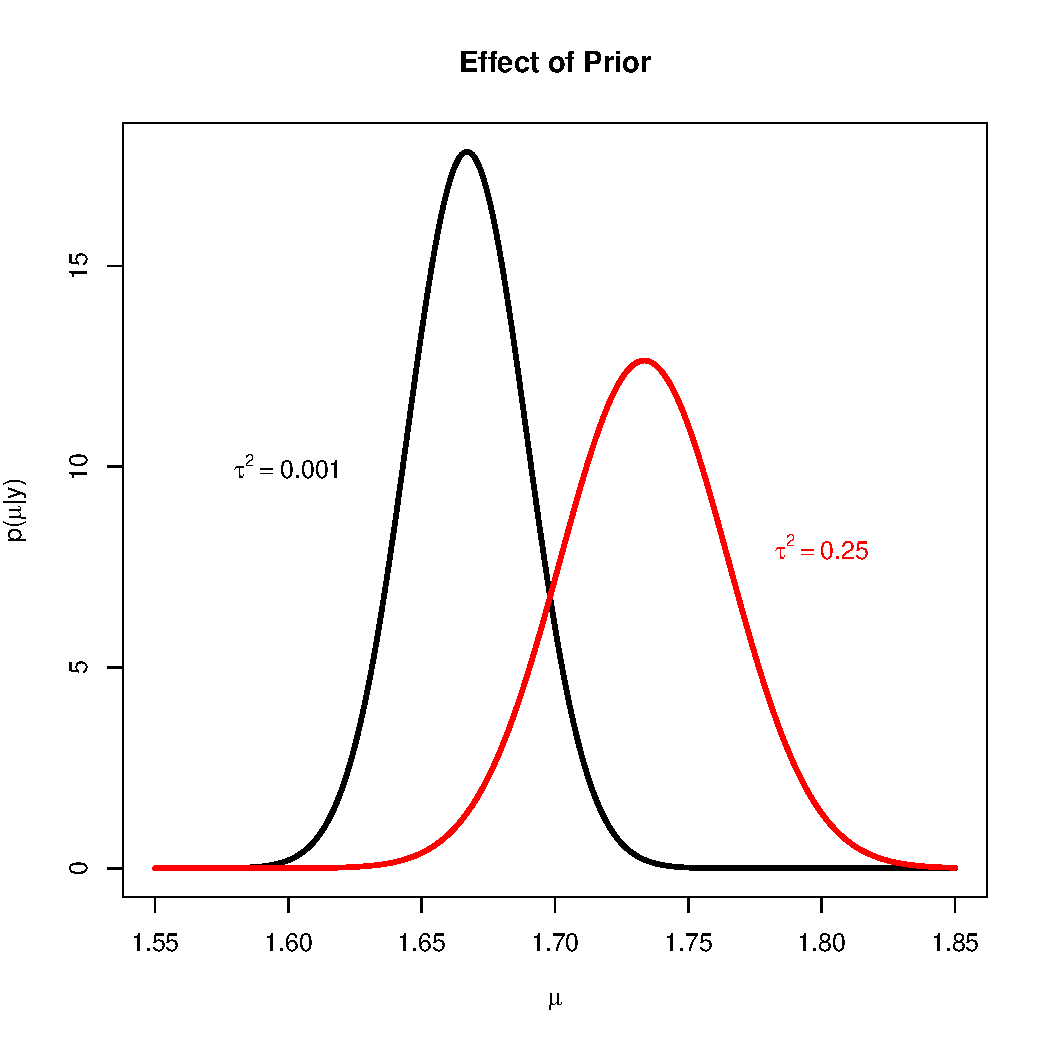
\includegraphics[height=7cm]{./Pics/compare1.pdf}
  \end{center}
\end{frame}
\begin{frame}{Let $\tau^2$ get big}
  \begin{itemize}
  \item In the limiting case where $\tau\rightarrow\infty$, the prior distribution becomes {\bf improper}

  \item In this limiting case $p(\mu)\propto k$ where $k$ is a constant.  This is called a {\bf flat prior}

  \item It can be verified that as $\tau\rightarrow\infty$, the posterior mean $a\rightarrow\sum y_i/n$ and $b\rightarrow \sigma^2/n$.

  \item When $p(\mu)\propto k$ $\mu|{\bm y}, \sigma^2\sim N(\sum y_i/n,\sigma^2/n)$

  \item This leads similar inference as in the classical case ($\sigma^2$ known).
  \end{itemize}
\end{frame}
\begin{frame}{Let $n$ get big}
  Now consider:
  \begin{itemize}
  \item $\sigma^2=0.01$
  \item $n=1000$
  \item $\sum y_i=1734$
  \item $\eta=1.6$
  \item $\tau^2=0.001$
  \end{itemize}
  What do you think happens when $n\rightarrow\infty$?
\end{frame}
\begin{frame}{Plot}
  \begin{center}
    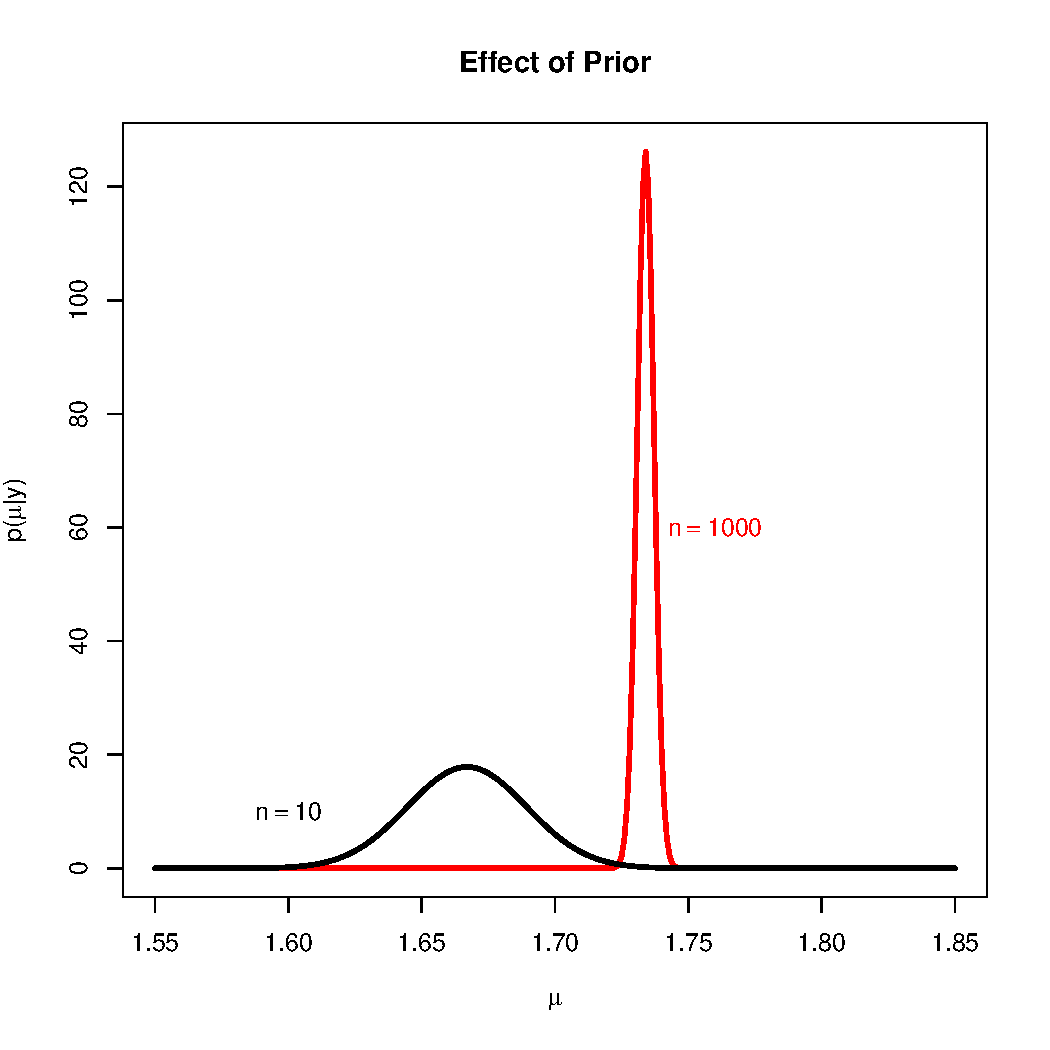
\includegraphics[height=7cm]{./Pics/compare2.pdf}
  \end{center}
\end{frame}
\begin{frame}{Summary}
  \begin{itemize}
  \item If the prior variance is large:

    \begin{itemize}
    \item The posterior mean will be closer to the sample mean.
    \item The posterior variance is larger.
    \end{itemize}

  \item If the prior variance is small:

    \begin{itemize}
    \item The posterior mean will be closer to the prior mean.
    \item The posterior variance is smaller.
    \end{itemize}

  \item As the sample size gets larger, prior information is dominated by the information in the likelihood.
  \end{itemize}
\end{frame}
\begin{frame}{More terminology}
  \begin{itemize}
  \item Improper prior: A prior that does not integrate to 1 for example the {\bf flat prior} $p(\mu)\propto 1$ where $\mu\in\mathbb{R}$

  \item Proper prior: A prior that does integrate to 1.

  \item Noninformative Prior: A prior that has a small effect on on the posterior.  It may be proper or improper

  \item Conjugate Prior: A prior that has the same distribution as the posterior
  \end{itemize}
\end{frame}
\begin{frame}{Examples of Conjugacy}
  \begin{itemize}
  \item Beta prior with Bernoulli likelihood give Beta posterior
    \begin{itemize}
    \item We say ``Beta is conjugate to the Bernoulli''.
    \end{itemize}

  \item Gaussian prior with Gaussian likelihood gives Gaussian posterior
    \begin{itemize}
    \item We say ``Gaussian is conjugate to the Gaussian''.
    \end{itemize}

  \item Gamma prior with Poisson likelihood gives Gamma posterior
    \begin{itemize}
    \item We say ``Gamma is conjugate to the Poisson''.
    \end{itemize}

  \item Not all priors are conjugate.
  \end{itemize}
\end{frame}
\section{Dealing with more than one parameter}
\begin{frame}{What about $\sigma^2$}
  \begin{itemize}
  \item In the previous section we ignored $\sigma^2$.

  \item The posterior we looked at was $p(\mu|\sigma^2,{\bm y})$

  \item In reality we also want to do inference on $\sigma^2$.

  \item Also since we have uncertainty about $\sigma^2$ it doesn't make sense to base inference on $p(\mu|\sigma^2,{\bm y})$
  \end{itemize}
\end{frame}
\begin{frame}{Inference is based on Marginal Posterior}
  \begin{itemize}
  \item Inference for $\mu$ will be based on

    \begin{equation}
      p(\mu|{\bm y})=\int_{\sigma^2}p(\mu,\sigma^2|{\bm y})d\sigma^2
    \end{equation}

  \item Similarly inference for $\sigma^2$ will be based on

    \begin{equation}
      p(\sigma^2|{\bm y})=\int_{\mu^2}p(\mu,\sigma^2|{\bm y})d\mu
    \end{equation}

  \item In both cases
    \begin{equation}
      p(\mu,\sigma^2|{\bm y})\propto p({\bm y}|\mu,\sigma^2)p(\mu,\sigma^2)
    \end{equation}
  \end{itemize}
\end{frame}
\begin{frame}{An interesting integral}
  \begin{itemize}
  \item Another way to write the integral for $p(\mu|{\bm y})$ is as

    \begin{equation*}
      \int_{\sigma^2}p(\mu,\sigma^2|{\bm y})d\sigma^2=
      \int_{\sigma^2}p(\mu|\sigma^2,{\bm y})p(\sigma^2|{\bm y})d\sigma^2
    \end{equation*}

  \item Here is should be  clear that we are `integrating' out or `averaging' out the uncertainty in $\sigma^2$

  \item The `weights' for this average are $p(\sigma^2|{\bm y})$

  \item The same applies to $\int_{\mu}p(\mu,\sigma^2|{\bm y})d\mu$
  \end{itemize}
\end{frame}
\begin{frame}{How do we do the integration?}
  \begin{itemize}
  \item In many cases integration can be done by {\bf recognising} a distribution.

  \item Let's consider the case where $p(\mu,\sigma^2)\propto (\sigma^2)^{-1}$

  \item This is the same as a flat prior on $\mu$ and a flat prior on $log(\sigma^2)$.

  \item We will find $p(\sigma^2|{\bm y})$
  \end{itemize}
\end{frame}
\begin{frame}{Two steps}
  \begin{enumerate}
  \item Recognize a distribution for $\mu$

    \begin{itemize}
    \item To make this integrate to 1 we must have normalizing constant.
    \item Also we cannot remove any terms involving $\sigma^2$
    \end{itemize}

  \item Recognize a distribution in $\sigma^2$
  \end{enumerate}
\end{frame}
\begin{frame}{Find posterior}
  \begin{align*}
    p(\sigma^2|{\bm y})&=\int_{\mu}p({\bm y}|\sigma^2,\mu)p(\sigma^2,\mu)d\mu\\
                       &\propto \int_{\mu}\left(\prod_{i=1}^n (2\pi\sigma^2)^{-1/2}
                         exp\left[-\frac{(y_i-\mu)^2}{2\sigma^2}\right]\right)(\sigma^{2})^{-1}d\mu\\
                       &\propto (2\pi\sigma^2)^{-n/2}(\sigma^{2})^{-1}\int_{\mu}\prod_{i=1}^n
                         exp\left[-\frac{(y_i-\mu)^2}{2\sigma^2}\right]d\mu\\
                       &\propto (\sigma^2)^{-\frac{n}{2}-1}\int_{\mu}\prod_{i=1}^n
                         exp\left[-\frac{(y_i-\mu)^2}{2\sigma^2}\right]d\mu\\
  \end{align*}
\end{frame}
\begin{frame}{The integral}
  Consider the integral
  \begin{equation}
    \int_{\mu}\prod_{i=1}^n
    exp\left[-\frac{(y_i-\mu)^2}{2\sigma^2}\right]d\mu
  \end{equation}
  With similar working as before we can show
  \begin{equation*}
    \int_{\mu}\prod_{i=1}^n
    exp\left[-\frac{(y_i-\mu)^2}{2\sigma^2}\right]d\mu=
    \int_{\mu}exp\left[-\frac{\sum(y_i^2)-2\mu\sum y_i+n\mu^2}{2\sigma^2}\right]d\mu
  \end{equation*}
\end{frame}
\begin{frame}
  \begin{align*}
    &=\int_{\mu}exp\left[-\frac{-2\mu\sum y_i+n\mu^2}{2\sigma^2}\right]
      exp\left[-\frac{\sum(y_i^2)}{2\sigma^2}\right]d\mu\\
    &=exp\left[-\frac{\sum(y_i^2)}{2\sigma^2}\right]\int_{\mu}exp\left[-\frac{-2\mu\bar{y}+\mu^2}{2(\sigma^2/n)}\right]
      d\mu\\
    &=exp\left[-\frac{\sum(y_i^2)}{2\sigma^2}\right]
      {\color{blue} exp\left[\frac{\bar{y}^2}{2(\sigma^2/n)}\right]}\times\\
    &\quad\quad
      \int_{\mu}exp\left[-\frac{{\color{blue}\bar{y}^2}-2\mu\bar{y}+\mu^2}{2(\sigma^2/n)}\right]
      d\mu\\
  \end{align*}
  where $\bar{y}=\sum y_i/n$
\end{frame}
\begin{frame}
  \begin{align*}
    &=exp\left[-\frac{\sum(y_i^2)-n\bar{y}^2}{2\sigma^2}\right]\times\\
    &\quad\quad
      \int_{\mu}exp\left[-\frac{(\mu-\bar{y})^2}{2(\sigma^2/n)}\right]
      d\mu\\
    &=exp\left[-\frac{\sum(y_i^2)-n\bar{y}^2}{2\sigma^2}\right]{\color{blue} \times(2\pi)^{1/2}(\sigma^2/n)^{1/2}}\times\\
    &\quad\quad
      \int_{\mu}{\color{blue}(2\pi)^{-1/2}(\sigma^2/n)^{-1/2}}exp\left[-\frac{(\mu-\bar{y})^2}{2(\sigma^2/n)}\right]
      d\mu\\
    &=exp\left[-\frac{\sum(y_i^2)-n\bar{y}^2}{2\sigma^2}\right]\times(2\pi)^{1/2}(\sigma^2)^{1/2}n^{-1/2}\\
  \end{align*}
\end{frame}
\begin{frame}{Back to the original aim}
  Now that $\mu$ has been integrated out we can focus on the posterior of $\sigma^2$
  \begin{align*}
    p(\sigma^2|{\bm y})&\propto (\sigma^2)^{-\frac{n}{2}-1}\int_{\mu}\prod_{i=1}^n
                         exp\left[-\frac{(y_i-\mu)^2}{2\sigma^2}\right]d\mu\\
                       &\propto (\sigma^2)^{-\frac{n}{2}-1}exp\left[-\frac{\sum(y_i^2)-n\bar{y}^2}{2\sigma^2}\right]\times(2\pi)^{1/2}(\sigma^2)^{1/2}n^{-1/2}\\
                       &\propto (\sigma^2)^{-\frac{(n-1)}{2}-1}exp\left[-\frac{\sum(y_i^2)-n\bar{y}^2}{2\sigma^2}\right]\\
  \end{align*}
  Can we recognise this?
\end{frame}
\begin{frame}{Inverse Gamma disribution}
  The kernel of the inverse Gamma disribution is given by
  \begin{equation}
    p(x)\propto x^{-a-1}exp(-b/x)
  \end{equation}
  We have
  \begin{equation}
    p(\sigma^2|{\bm y})\propto (\sigma^2)^{-\frac{(n-1)}{2}-1}exp\left[-\frac{\sum(y_i^2)-n\bar{y}^2}{2\sigma^2}\right]
  \end{equation}
  Match the parameters
\end{frame}
\begin{frame}
  \begin{itemize}
  \item The posterior is

    \begin{equation}
      \sigma^2|{\bm y}\sim IG\left(\frac{n-1}{2},\frac{\sum(y_i^2)-n\bar{y}^2}{2}\right)
    \end{equation}

  \item All inference on the mean is based on this distribution.

  \item A point estimate can be given by $E_{\sigma^2|{\bm y}}[\sigma^2]=\frac{\sum(y_i^2)-n\bar{y}^2}{n-2}$.

  \item Credible intervals for the mean can also be found.

  \item We can do a similar process to show that the posterior $p(\mu|{\bm y})$ follows a Student t distribution.
  \end{itemize}
\end{frame}
\begin{frame}{This is annoying}
  \begin{itemize}
  \item Integrating out the parameters involves tedious mathematics.

  \item Even worse in some cases it does not even lead to a posterior that we can recognize.

  \item For example, for the prior $\mu\sim N(\eta,\tau^2)$, then p($\sigma^2|{\bm y})$ not Inverse Gamma.  It is {\bf unrecognizable}

  \item What can we do?
  \end{itemize}
\end{frame}
\section{MCMC and Bayesian Inference}
\begin{frame}{Markov chain Monte Carlo}
  \begin{itemize}
  \item Although we cannot recognize the posterior, we do know the density.

  \item We may only know the kernel of the density and not the normalizing constant.

  \item Is it possible to at least draw a sample from the joint posterior?
  \end{itemize}
\end{frame}
\begin{frame}{Inference by MCMC}
  \begin{itemize}
  \item Consider the case where $p(\mu,\sigma^2)=p(\mu)p(\sigma^2)$ where

    \begin{itemize}
    \item $\mu\sim N(\eta,\tau^2)$
    \item $p(\sigma^2)\propto (\sigma^2)^{-1}$
    \end{itemize}

  \item In this case the posterior of $\mu$ is:

    \begin{equation}
      p(\mu|{\bm y})\propto
      \left[\sum (y_i-\mu)^2\right]^{-n/2}
      exp\left[-\frac{(\mu-\eta)^2}{2\tau^2}\right]
      \label{eq:tar}
    \end{equation}

  \item This cannot be recognized.
  \end{itemize}
\end{frame}
\begin{frame}{Metropolis Algorithm}
  \begin{itemize}
  \item Use the Metropolis algorithm to simulate a sample from $\mu|{\bm y}$ where the target density is given by Equation~\ref{eq:tar}.

  \item Use the values:
    \begin{itemize}
    \item $n=10$
    \item $\sum y_i=17.34$
    \item $\sum y^2_i=32$
    \item $\eta=1.8$
    \item $\tau^2=0.25$
    \end{itemize}

  \item Make a Monte Carlo approximation of $E[\mu|{\bm y}]$
  \end{itemize}
\end{frame}
\begin{frame}{Summary}
  \begin{itemize}
  \item Bayesian Inference treats all unknown quantities including parameters as {\bf random variables}

  \item All inference is based on the {\bf posterior}

  \item In some cases the posterior can be evaluated and recognized.

  \item In other cases algorithms such as the Metropolis algorithm can be used.

  \item Next week we will look at improvements on the basic Metropolis algorithm.
  \end{itemize}
\end{frame}
\end{document}
